\chapter{ITOLABMOTORDRIVER 電子部品リスト}
\begin{tabular}{|c|c|c|c|} \hline
 &部品名&型番&PDF URL\\ \hline
 1&4P,EIコネクタピンヘッダ&171825-4-50P&\url{https://jp.misumi-ec.com/}\\
 &                       &            &\url{pdf/el/2015_H/0380.pdf}\\ \hline
2&回生ダイオード&20ETS12FP&\url{http://akizukidenshi.com/}\\
 &              &         &\url{download/ds/vishay/}\\
 &              &         &\url{vs20ets.pdf}\\ \hline
3&ターミナルブロック&P-02333&\url{http://akizukidenshi.com/}\\
 &                  &       &\url{download/ds/alphaplus/TB}\\
 &                  &       &\url{111-2-x-x-x-x.pdf}\\ \hline
4&カーボン被膜抵抗&R-25103&\url{http://akizukidenshi.com/}\\
 &10kΩ&       &\url{download/ds/faithful/}\\
 &     &       &\url{R1_CF.pdf}\\ \hline
5&カーボン被膜抵抗&R-25103&\url{http://akizukidenshi.com/}\\
 &47kΩ&       &\url{download/ds/faithful/}\\
 &     &       &\url{R1_CF.pdf}\\ \hline
6&カーボン被膜抵抗&R-25470&\url{http://akizukidenshi.com/}\\
 &47Ω&       &\url{download/ds/faithful/}\\
 &    &       &\url{R1_CF.pdf}\\ \hline
7&汎用小信号高速&1N4148&\url{http://akizukidenshi.com/}\\
 &スイッチング・ダイオード&      &\url{download/1n4148.pdf}\\ \hline
8&セラミックコンデンサ&P-00090&\url{http://akizukidenshi.com/}\\
 &0.1μ&       &\url{download/ds/murata/}\\
 &     &       &\url{RPEF11H104Z2P1A01B_a.pdf}\\ \hline
9&セラミックコンデンサ&P-03095&\url{http://akizukidenshi.com/}\\
 &10μ&        &\url{download/rd_series.pdf}\\ \hline
\end{tabular}
\begin{tabular}{|c|c|c|c|} \hline
10&ハーフブリッジドライバ&IR2302PBF&\url{http://akizukidenshi.com/}\\
  &8-DIP&    &\url{download/ds/ir/ir2302.pdf}\\ \hline
11&ピンソケット&c-03951&\url{http://akizukidenshi.com/}\\
  &14×2P&    &\url{download/ds/kakusya/}\\
  &      &    &\url{FH-2X00SG.pdf}\\ \hline
12&RX200マイコンボード&K-08769&\url{http://akizukidenshi.com/}\\
  &                   &       &\url{download/ds/akizuki/}\\
  &                   &       &\url{RX220_CPU_Manual.pdf}\\ \hline
13&トロイダルコイル&P-06731&\url{http://akizukidenshi.com/}\\
  &330μH9A&     &\url{download/ds/core/}\\
  &        &     &\url{TCV-331M-9A-8026.pdf}\\ \hline
14&NchパワーMOSFET&EKI04047&\url{http://akizukidenshi.com/}\\
  &               &        &\url{download/ds/sanken/}\\
  &               &        &\url{eki04047_ds_en.pdf}\\ \hline
\end{tabular}

\chapter{新高出力モータドライバ 電子部品リスト}
\begin{tabular}{|c|c|c|c|} \hline
 &部品名&型番&PDF URL\\ \hline
 1&4P,EIコネクタピンヘッダ&171825-4-50P&\url{https://jp.misumi-ec.com/}\\
 &                       &            &\url{pdf/el/2015_H/0380.pdf}\\ \hline
2&回生ダイオード&20ETS12FP&\url{http://akizukidenshi.com/}\\
 &              &         &\url{download/ds/vishay/}\\
 &              &         &\url{vs20ets.pdf}\\ \hline
3&ターミナルブロック&P-02333&\url{http://akizukidenshi.com/}\\
 &                  &       &\url{download/ds/alphaplus/TB}\\
 &                  &       &\url{111-2-x-x-x-x.pdf}\\ \hline
4&カーボン被膜抵抗&R-25103&\url{http://akizukidenshi.com/}\\
 &10kΩ&       &\url{download/ds/faithful/}\\
 &     &       &\url{R1_CF.pdf}\\ \hline
5&カーボン被膜抵抗&R-25103&\url{http://akizukidenshi.com/}\\
 &47kΩ&       &\url{download/ds/faithful/}\\
 &     &       &\url{R1_CF.pdf}\\ \hline
6&カーボン被膜抵抗&R-25470&\url{http://akizukidenshi.com/}\\
 &47Ω&       &\url{download/ds/faithful/}\\
 &    &       &\url{R1_CF.pdf}\\ \hline
7&汎用小信号高速&1N4148&\url{http://akizukidenshi.com/}\\
 &スイッチング・ダイオード&      &\url{download/1n4148.pdf}\\ \hline
8&セラミックコンデンサ&P-00090&\url{http://akizukidenshi.com/}\\
 &0.1μ&       &\url{download/ds/murata/}\\
 &     &       &\url{RPEF11H104Z2P1A01B_a.pdf}\\ \hline
9&セラミックコンデンサ&P-03095&\url{http://akizukidenshi.com/}\\
 &10μ&        &\url{download/rd_series.pdf}\\ \hline
\end{tabular}
\begin{tabular}{|c|c|c|c|} \hline
10&ハーフブリッジドライバ&IR2302PBF&\url{http://akizukidenshi.com/}\\
  &8-DIP&    &\url{download/ds/ir/ir2302.pdf}\\ \hline
11&ピンソケット&c-03951&\url{http://akizukidenshi.com/}\\
  &14×2P&    &\url{download/ds/kakusya/}\\
  &      &    &\url{FH-2X00SG.pdf}\\ \hline
12&RX200マイコンボード&K-08769&\url{http://akizukidenshi.com/}\\
  &                   &       &\url{download/ds/akizuki/}\\
  &                   &       &\url{RX220_CPU_Manual.pdf}\\ \hline
13&トロイダルコイル&P-06731&\url{http://akizukidenshi.com/}\\
  &330μH9A&     &\url{download/ds/core/}\\
  &        &     &\url{TCV-331M-9A-8026.pdf}\\ \hline
14&NchパワーMOSFET&EKI04047&\url{http://akizukidenshi.com/}\\
  &               &        &\url{download/ds/sanken/}\\
  &               &        &\url{eki04047_ds_en.pdf}\\ \hline
15&3mm 砲弾型LED&I-09851&\url{http://akizukidenshi.com/}\\
  &             &       &\url{download/ds/lg/}\\
  &&&\url{LEBWL34A06AA00.pdf}\\ \hline
16&タクトスイッチ&TVDP01-060CB&\url{http://akizukidenshi.com/}\\
&&&\url{download/ds/cosland/}\\
&&&\url{DTS-6-V.PDF}\\ \hline
17&温度センサ&MCP9700&\url{http://akizukidenshi.com/}\\
&&&\url{download/MCP9701-ETO.pdf}\\ \hline
18&電流センサ&ACS758LCB-100B&\url{https://www.digikey.jp/}\\
&&&\url{product-detail/}\\
&&&\url{ja/allegro-microsystems-llc/}\\
&&&\url{ACS758LCB-100B-PFF-T/}\\
&&&\url{620-1321-ND/2042746}\\ \hline
19&RS485トランシーバ&LT1785CN8&\url{http://akizukidenshi.com/}\\
&&&\url{download/lt1785cn8.pdf}\\ \hline
\end{tabular}

\chapter{ロボコン用高出力モータドライバ回路図}
\newpage
\begin{figure}[H]
\begin{center}
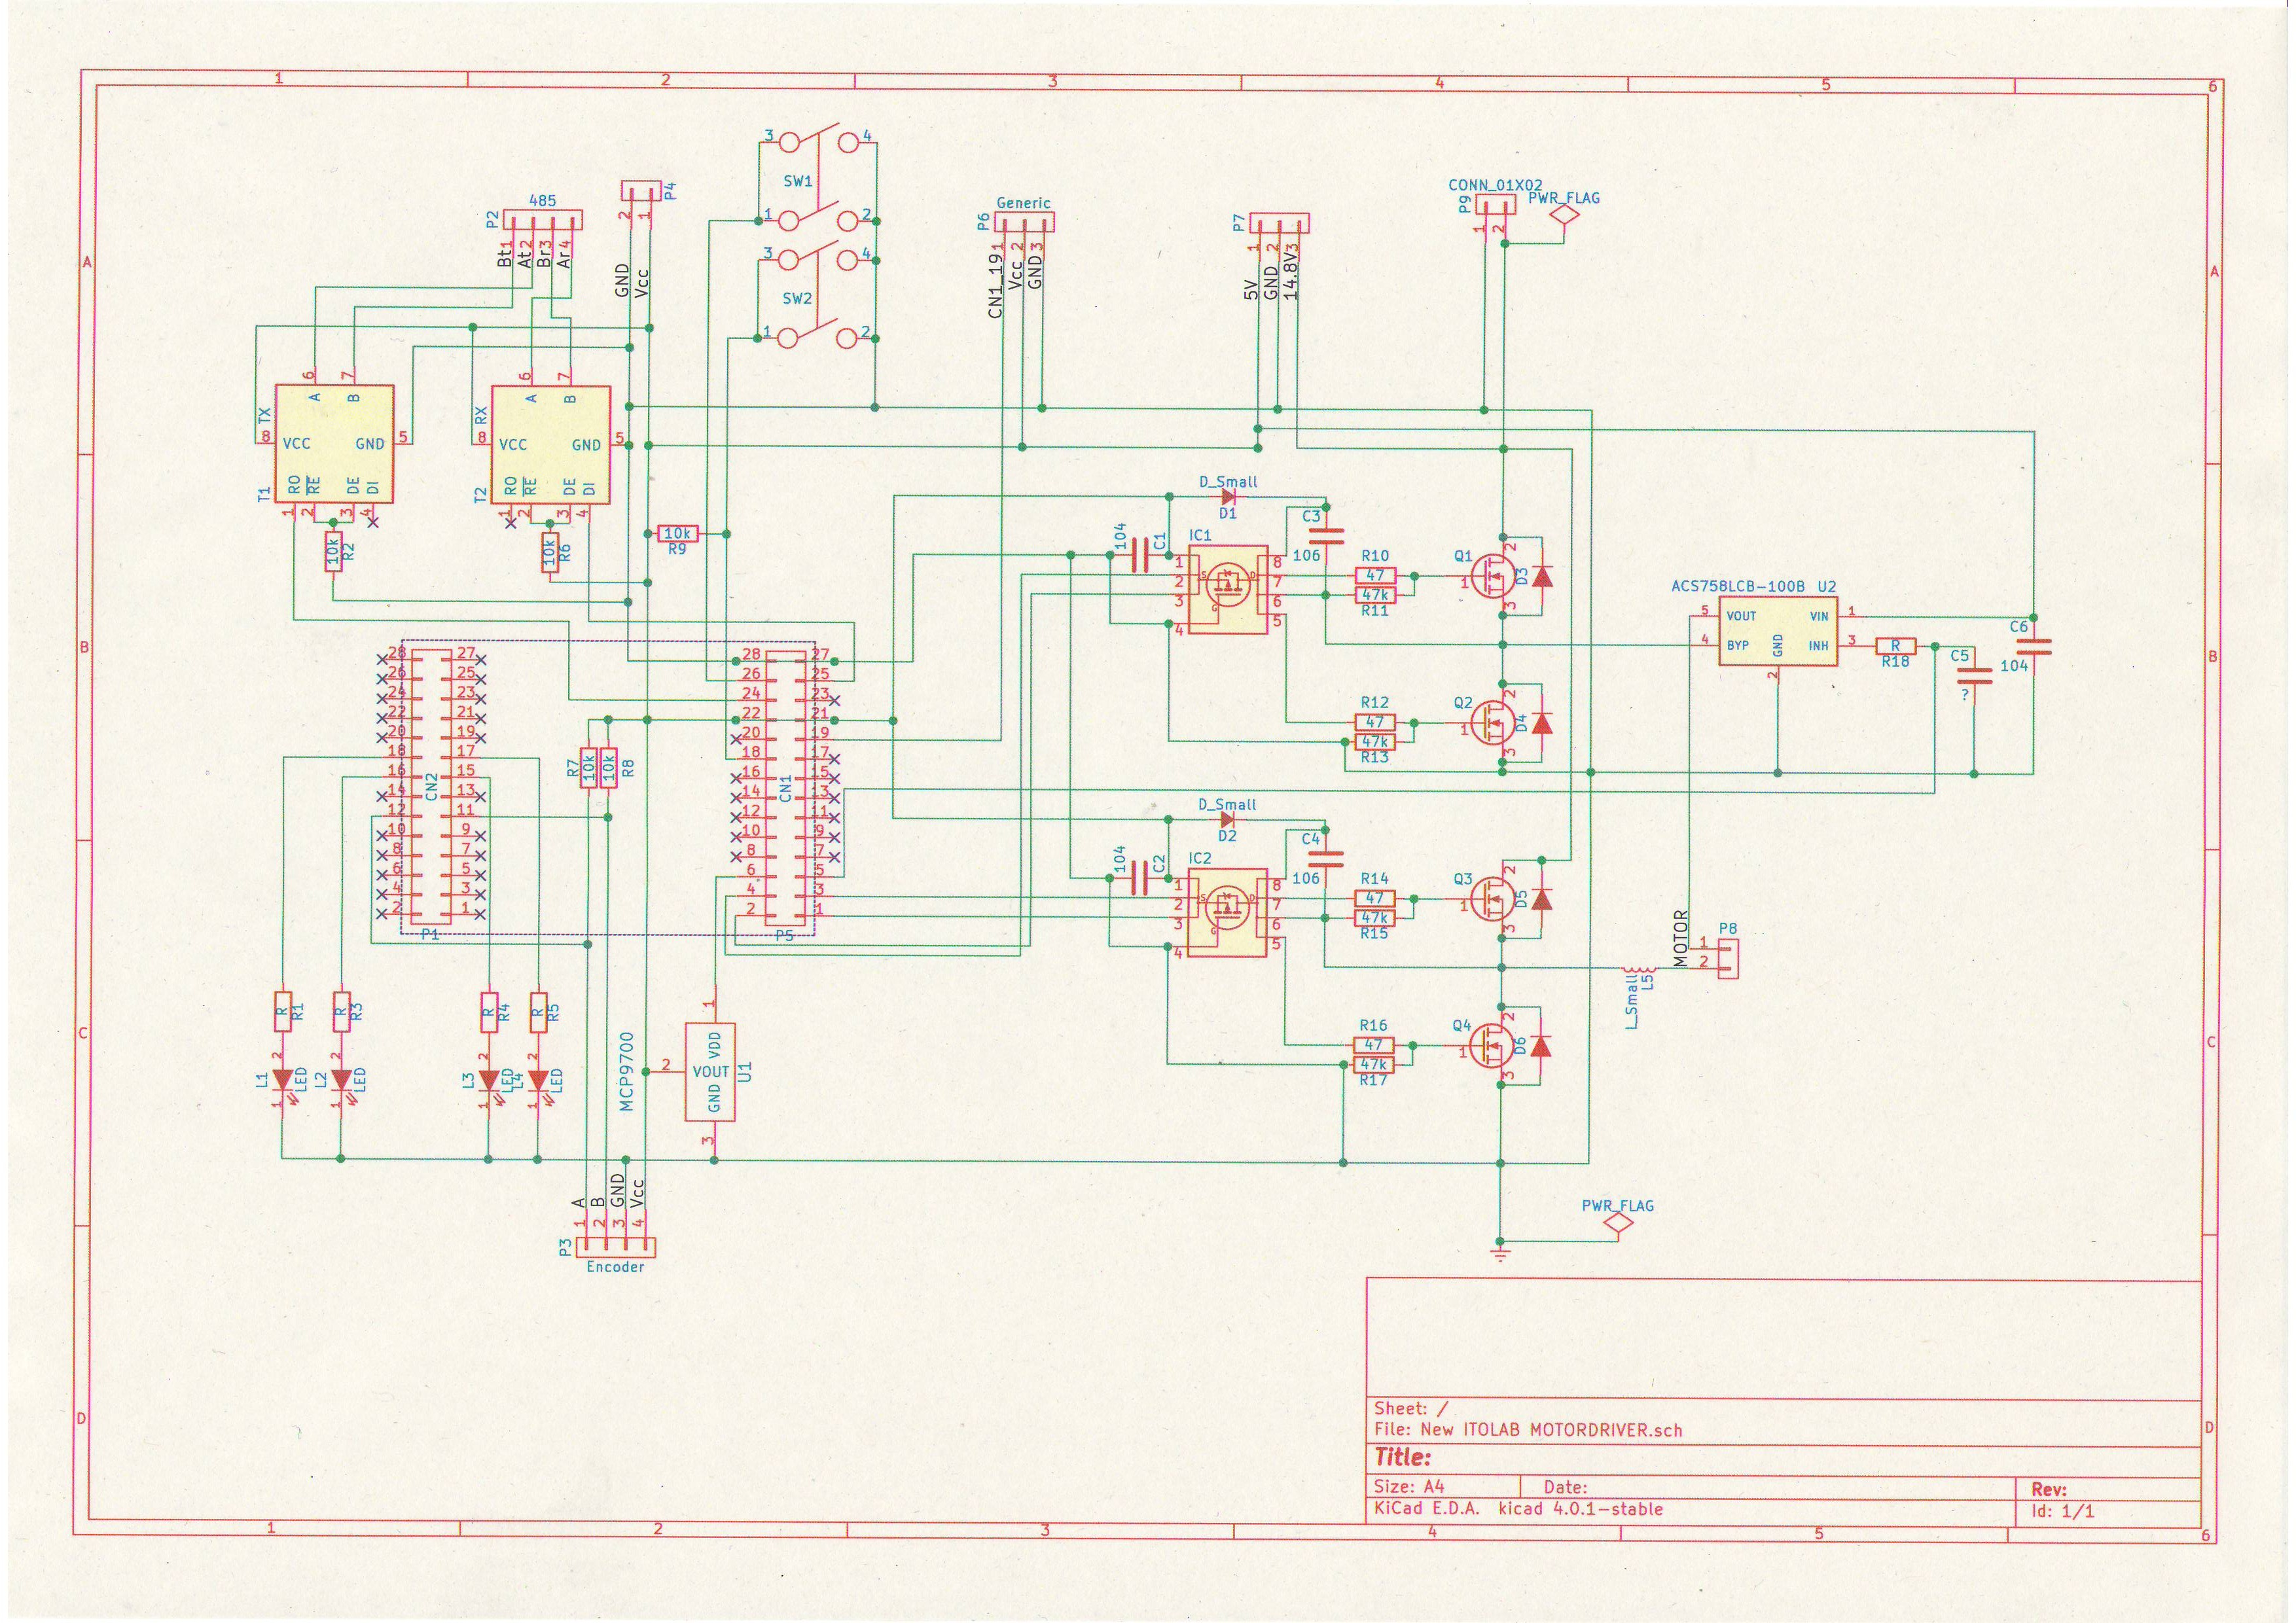
\includegraphics[width=200mm, angle=90]{kairozu2}
\end{center}
\caption{回路図}
\label{fig:kairozu2}
\end{figure}

\chapter{RXマイコンと各部品との接続}
\begin{tabular}{|c|c|c|} \hline
ピンNo.   &ポート番号&接続先           \\ \hline \hline
CN1-1     &P4-0(出力)&右ゲート ローサイド\\ \hline
CN1-2     &P4-1(出力)&左ゲート ローサイド\\ \hline
CN1-3     &P4-2(出力)&右ゲート ハイサイド\\ \hline
CN1-4     &P4-3(出力)&左ゲート ハイサイド\\ \hline
CN1-5     &P4-4(入力)&      電流センサ \\ \hline
CN1-6     &P4-6(入力)&      温度センサ \\ \hline
CN1-18    &PO-3(入力)&    汎用スイッチ \\ \hline
CN1-19    &PO-5(入力/出力)&      汎用ポート \\ \hline
CN1-21    &          &              5V \\ \hline
CN1-22    &          &              5V \\ \hline
CN1-24    &RS232(RXD)&          TX信号 \\ \hline
CN1-25    &RS232(TXD)&          RX信号 \\ \hline
CN1-26    &RES#     &リセットスイッチ \\ \hline
CN1-27    &          &             GND \\ \hline
CN1-28    &          &             GND \\ \hline \hline
CN2-11    &MTCLKA    &エンコーダB\\ \hline
CN2-12    &MTCLKB    &エンコーダA\\ \hline
CN2-15    &PH-0(出力)&汎用LED    \\ \hline
CN2-16    &PH-1(出力)&汎用LED    \\ \hline
CN2-17    &PH-2(出力)&汎用LED    \\ \hline
CN2-18    &PH-3(出力)&汎用LED    \\ \hline
\end{tabular}

\chapter{KiCadの使い方}
\begin{enumerate}
\item KiCadのホームから,図\ref{fig:1k-h}のように回路図エディタを開く.
\begin{figure}[H]
  \begin{center}
    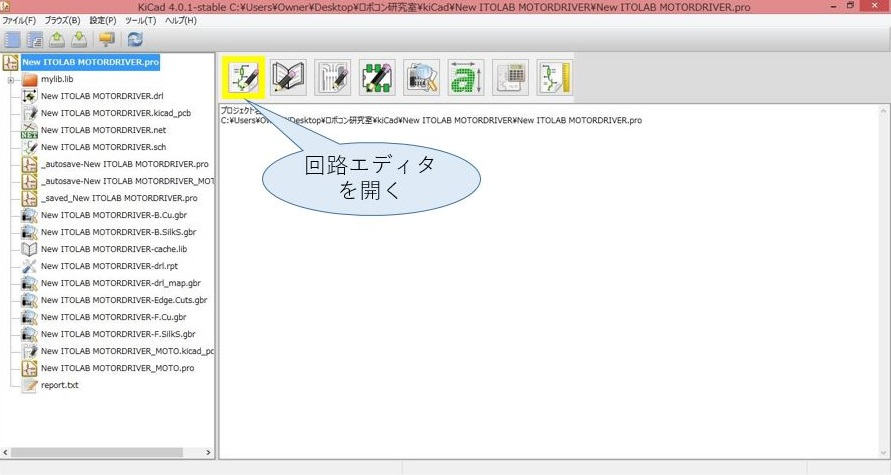
\includegraphics[width=150mm]{1k-h}
    \end{center}
  \caption{ホーム画面}
 \label{fig:1k-h}
\end{figure}
\item 回路エディタで,図\ref{fig:2k-m}のように電子部品,電源,配線を選択して回路図を
作成する.
\begin{figure}[H]
  \begin{center}
    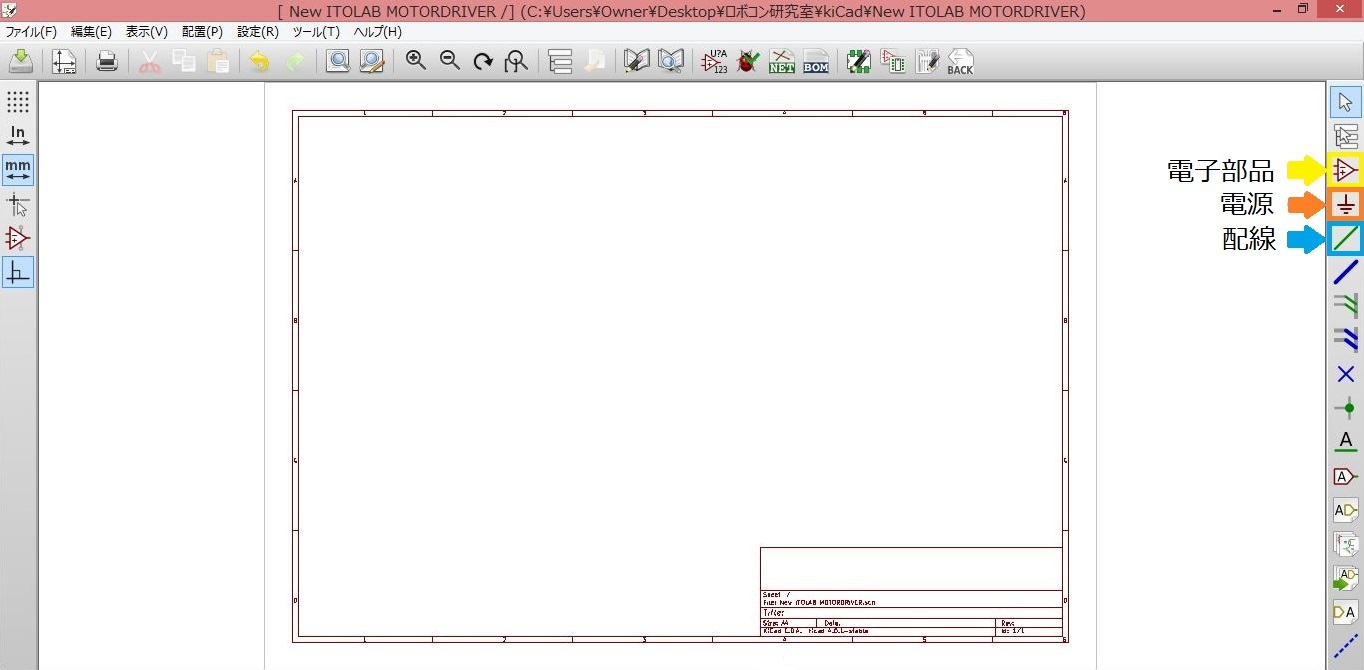
\includegraphics[width=150mm]{2k-m}
    \end{center}
  \caption{回路エディタ}
 \label{fig:2k-m}
\end{figure}
\item 回路図作成後,図\ref{fig:3m}のようにネットリストの作成を行う.
\begin{figure}[H]
  \begin{center}
    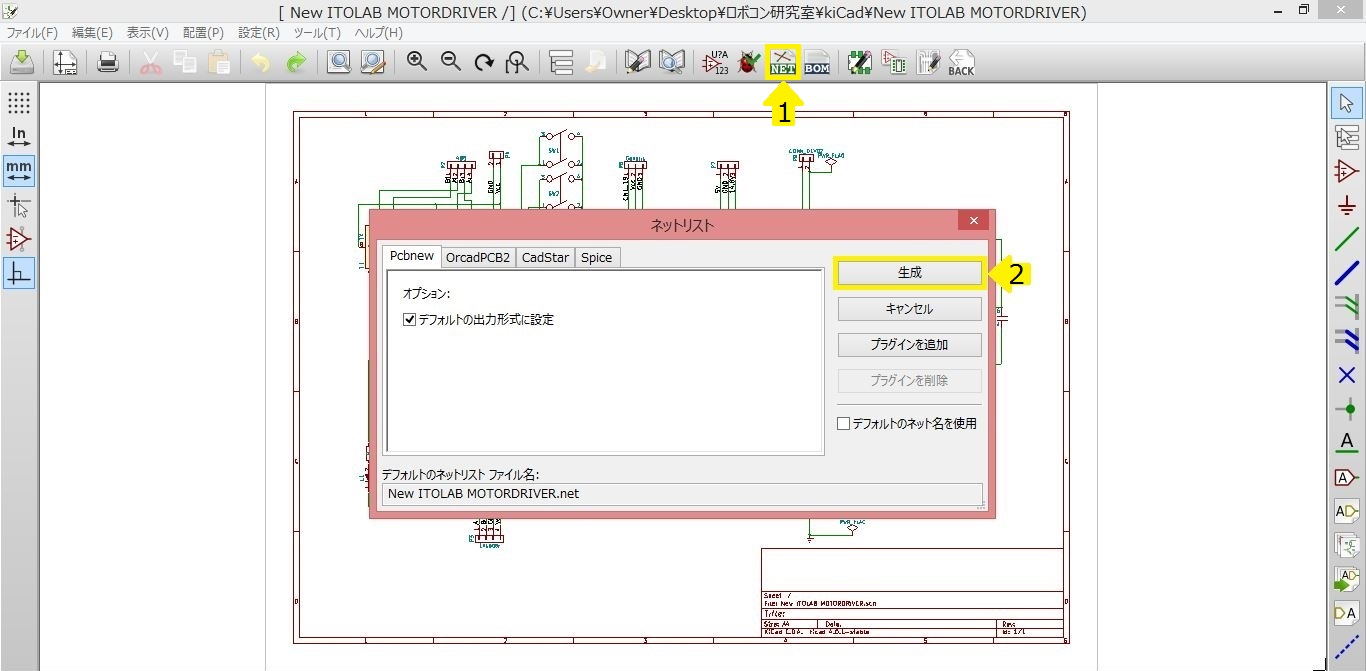
\includegraphics[width=150mm]{3m}
    \end{center}
  \caption{回路エディタ}
 \label{fig:3m}
\end{figure}
\item 図\ref{fig:4n}のようにしてコンポーネントとフットプリントの関連付けを行う.
\begin{figure}[H]
  \begin{center}
    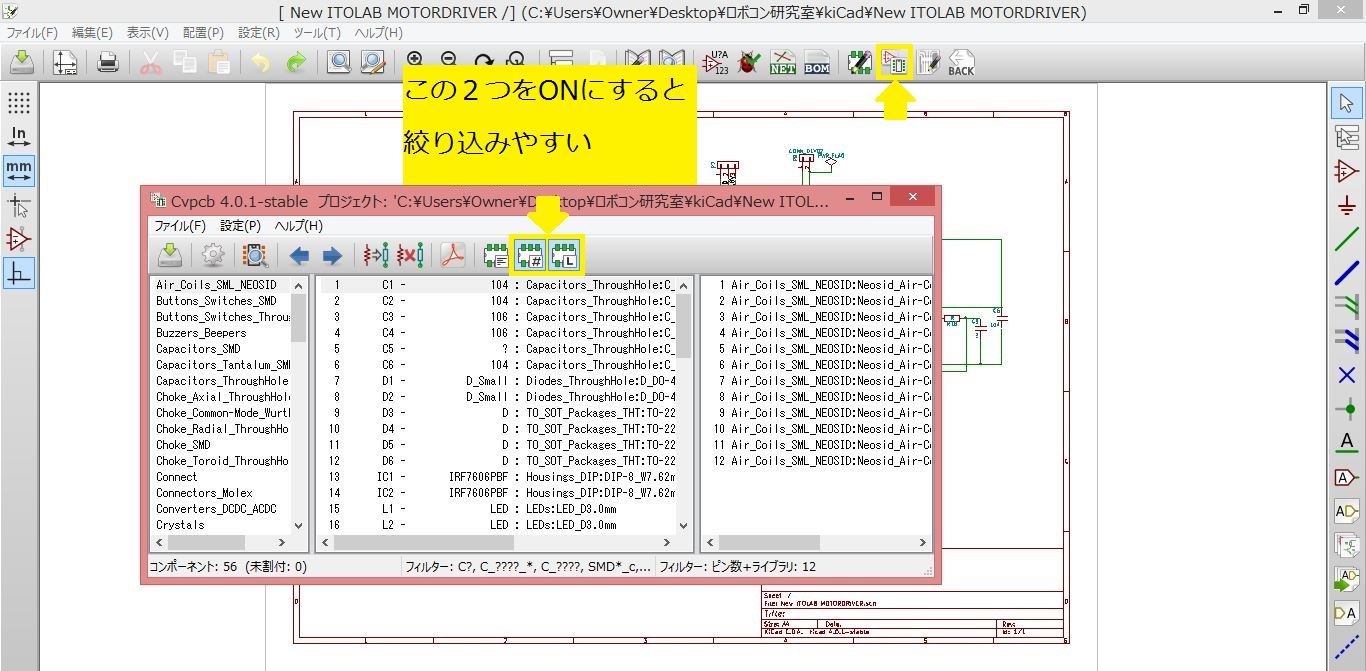
\includegraphics[width=150mm]{4n}
    \end{center}
  \caption{回路エディタ}
 \label{fig:4n}
\end{figure}
\item 図\ref{fig:5o}のように,アイコンをクリックしてプリント基板のレイアウトの
実行を行う.
\begin{figure}[H]
  \begin{center}
    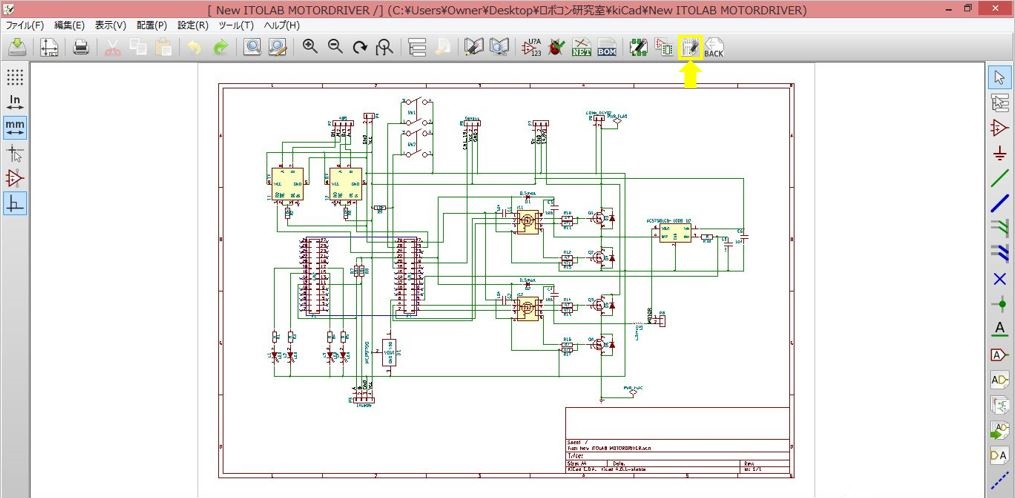
\includegraphics[width=150mm]{5o}
    \end{center}
  \caption{基板レイアウトの実行}
 \label{fig:5o}
\end{figure}
\item 図\ref{fig:6j}のようにして,ネットリストを読み込む.
\begin{figure}[H]
  \begin{center}
    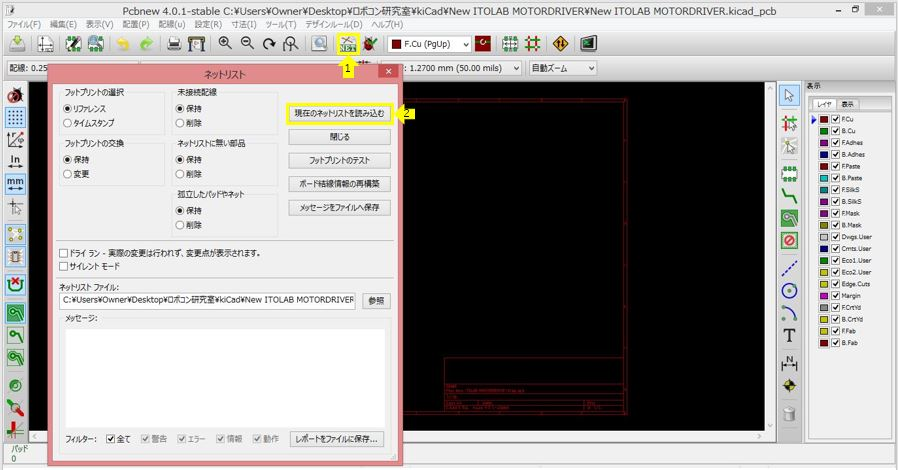
\includegraphics[width=150mm]{6j}
    \end{center}
  \caption{ネットリストの読み込み}
 \label{fig:6j}
\end{figure}
\item 図\ref{fig:7b}のように部品が表示されるので,部品をきれいに配置する.
\begin{figure}[H]
  \begin{center}
    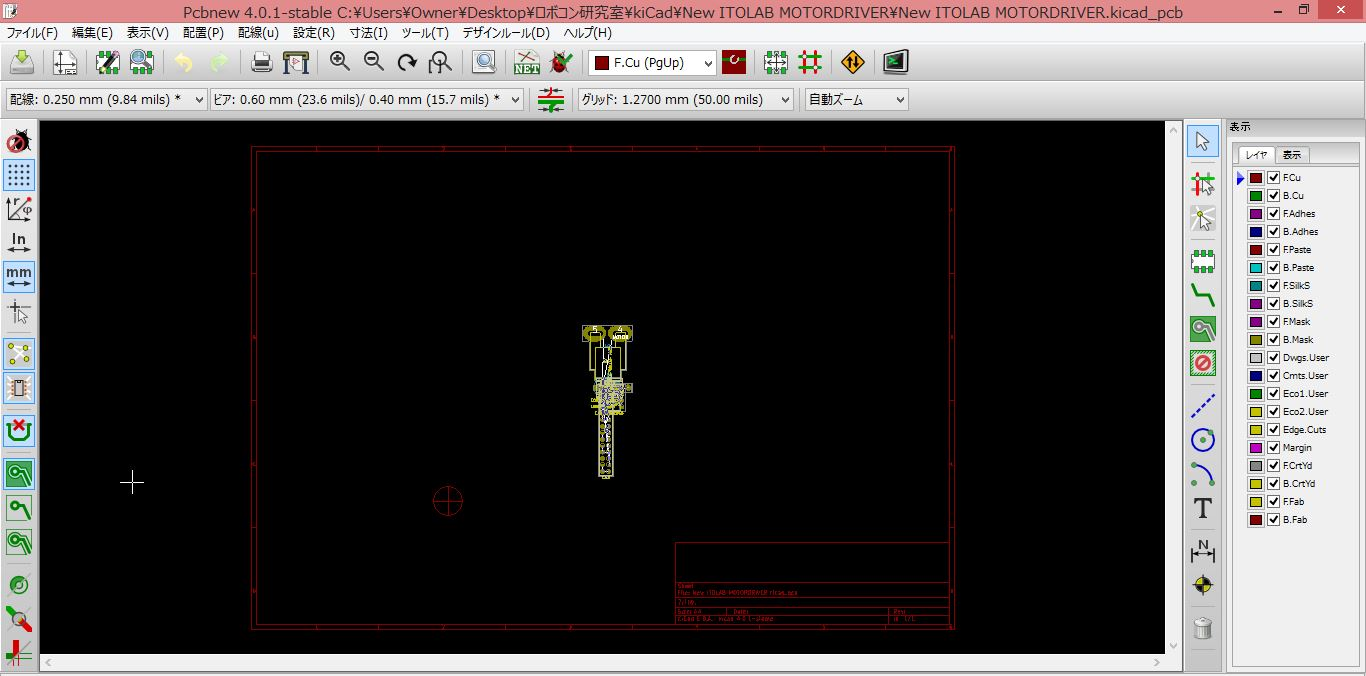
\includegraphics[width=150mm]{7b}
    \end{center}
  \caption{表示された部品}
 \label{fig:7b}
\end{figure}
\item 図\ref{fig:8b}のように,配線,基板枠の作成を行う.
\begin{figure}[H]
  \begin{center}
    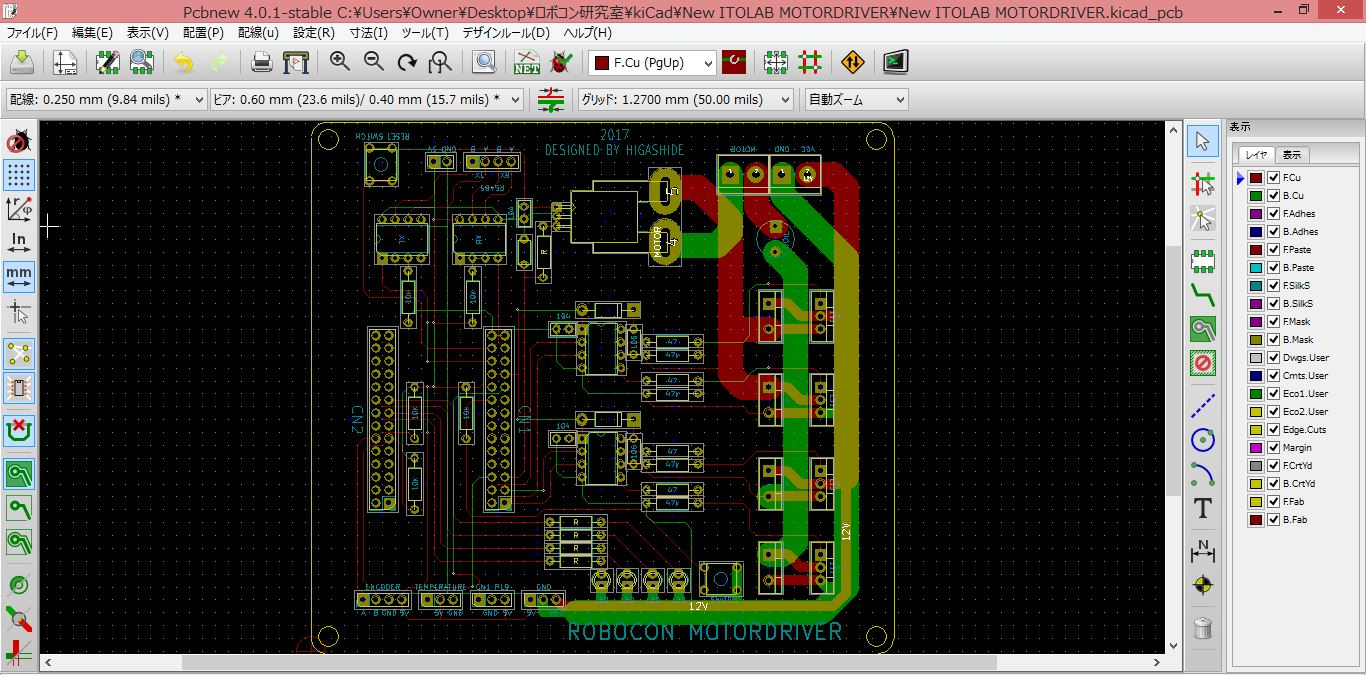
\includegraphics[width=150mm]{8b}
    \end{center}
  \caption{配線後}
 \label{fig:8b}
\end{figure}
\item 図\ref{fig:9b}のように,GNDをベタにする.
\begin{figure}[H]
  \begin{center}
    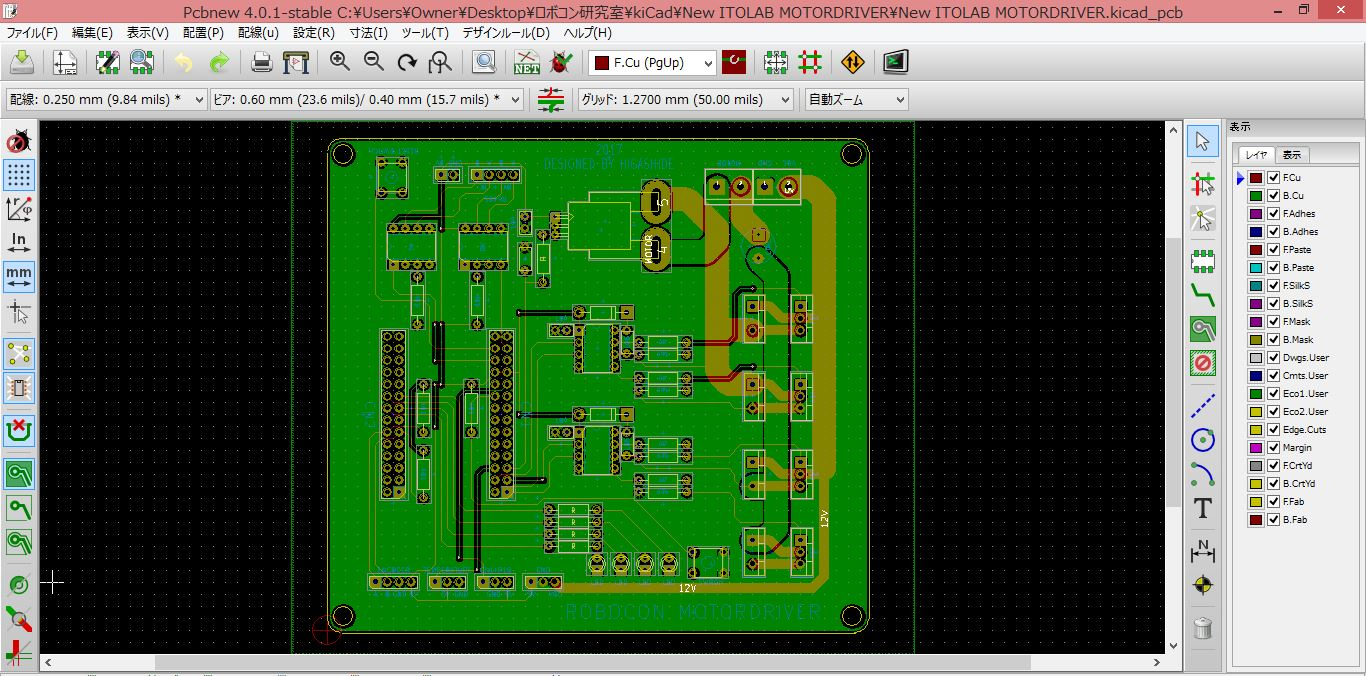
\includegraphics[width=150mm]{9b}
    \end{center}
  \caption{GNDベタ}
 \label{fig:9b}
\end{figure}
\end{enumerate}

\chapter{温度センサのデータシート}
\includepdf[pages=-]{ronbun2.pdf}
\chapter{電流センサのデータシート}
\includepdf[pages=-]{ronbun3.pdf}
\chapter{RS485トランシーバのデータシート}
\includepdf[pages=-]{ronbun4.pdf}
\chapter{FETのデータシート}
\includepdf[pages=-]{ronbun5.pdf}
\chapter{ハーフブリッジドライバのデータシート}
\includepdf[pages=-]{ronbun6.pdf}
